\chapter{Theoretische Grundlagen}

\section{Phishing-Webseiten als Anwendungsdomäne}
\subsection{Phishing und Social Engineering}

Phishing nutzt betrügerische E-Mails und Webseiten, um sensible Informationen zu erlangen; dazu können legitime Webseiten kopiert und für die Datenerfassung verändert werden (vgl. [Zhang et al. (2007), PDF-S. 1 und 3]). Die Täuschung beruht unter anderem darauf, dass Nutzer visuelle Inhalte als glaubwürdig wahrnehmen (vgl. [Dhamija et al. (2006), PDF-S. 1]).

Dhamija et al. untersuchten 22 Teilnehmende anhand von 20 Webseiten: 23 Prozent berücksichtigten browserbasierte Hinweise wie Adressleiste, Statusleiste oder Sicherheitsindikatoren nicht; die überzeugendste Phishing-Webseite täuschte 90 Prozent der Teilnehmenden (vgl. [Dhamija et al. (2006), PDF-S. 1]). Diese kleine Studie veranschaulicht die Täuschungswirkung, erlaubt aber keine Schätzung heutiger Erfolgsraten.

ENISA nennt Phishing für Juli 2024 bis Juni 2025 als häufigsten initialen Angriffsvektor und ordnet der breit gefassten Kategorie einschließlich Vishing, Malspam und Malvertising rund 60 Prozent der ausgewerteten Eintrittswege zu (vgl. [ENISA (2025a), S. 8]). Der Anteil bezieht sich somit nicht allein auf Phishing-Webseiten. Phishing-as-a-Service-Angebote erleichtern auch weniger versierten Akteuren die Durchführung von Kampagnen, etwa durch automatisiert erstellte Phishing-Kits und nachgebildete Anmeldeseiten (vgl. [ENISA (2025a), S. 11]).

Für den europäischen Finanzsektor wertete ENISA 488 öffentlich berichtete Sicherheitsvorfälle von Januar 2023 bis Juni 2024 aus; Kreditinstitute bildeten mit 46~\% die am häufigsten betroffene Gruppe (vgl. [ENISA (2025b), S.~3]). Phishing, Smishing und Vishing richteten sich gegen Institute und Kunden; bei 36~\% der betrachteten Social-Engineering-Vorfälle wurden primär Kreditinstitute imitiert (vgl. [ENISA (2025b), S.~13]).

Phishing-Webseiten können somit in unterschiedlichen inhaltlichen und technischen Ausprägungen auftreten. Für ihre automatisierte Erkennung sind insbesondere die unmittelbar auswertbaren Eigenschaften der URL und des HTML-Dokuments relevant, die im folgenden Abschnitt näher betrachtet werden.

\subsection{URL-, HTML-Text- und DOM-Daten als Informationsgrundlage}
URL und HTML-Dokument liefern unterschiedliche Informationen über dieselbe Webseite: Die URL beschreibt deren Adresse, der HTML-Inhalt ergänzt semantische und strukturelle Eigenschaften (vgl. [Opara et al. (2024), S. 2]). Die Arbeit nutzt diese Informationsquellen in getrennten Modellzweigen.

Yoon et al. verarbeiten URLs sowohl als numerisch repräsentierte Zeichenfolgen als auch über eine wortbasierte Darstellung (vgl. [Yoon et al. (2024), S. 6--7]). Die URL kann damit unabhängig vom HTML-Inhalt als sequenzielle Eingabe dienen.

Die Beziehungen zwischen HTML-Elementen lassen sich als Document Object Model (DOM) abbilden; Yoon et al. kombinieren einen HTML-DOM-Graphen mit URL-Repräsentationen (vgl. [Yoon et al. (2024), S. 2]). Im Folgenden werden entsprechend der textuelle HTML-Inhalt und die strukturelle DOM-Repräsentation unterschieden.

\subsection{Herausforderungen der automatisierten Erkennung}

Veränderungen von Phishing-Webseiten können die Übertragbarkeit zuvor trainierter Modelle einschränken (vgl. [Purwanto et al. (2022), S. 1498]). Eine hohe Leistung auf datensatznahen Testdaten genügt daher nicht als Nachweis der Erkennung zukünftiger Webseiten.

Ähnliche Instanzen in Training und Test können die gemessene Generalisierungsleistung begünstigen (vgl. [Dalton et al. (2026), S. 3]). Die Evaluation dieser Arbeit berücksichtigt deshalb zeitliche und strukturelle Trennungen. Zusätzlich wird die Erkennung bei niedriger False-Positive-Rate betrachtet, einem für die Phishing-Erkennung relevanten Betriebspunkt (vgl. [Purwanto et al. (2022), S. 1506]).

Auch im operativen Sicherheitsbetrieb zählt die False-Positive-Rate zu den Qualitätskennzahlen
von Security Operations Centers und wird neben Kennzahlen wie der Anzahl von Eskalationen und
dem Bearbeitungsaufwand pro Sicherheitsvorfall betrachtet
(vgl. [ENISA (2020), S. 7]). Dieser Aspekt ist vor dem Hintergrund begrenzter betrieblicher
Ressourcen besonders relevant, da fehlende Budgets und ein Mangel an
IT-Sicherheitsspezialisten zu den identifizierten Herausforderungen kleiner und mittlerer
Unternehmen zählen (vgl. [ENISA (2021), S. 14]).

Task-Adaptive Pretraining setzt das selbstüberwachte Vortraining auf ungelabelten Trainingsdaten einer konkreten Downstream-Aufgabe fort und kann deren Leistung verbessern (vgl. [Gururangan et al. (2020), S. 8346--8347]). Dies motiviert die Untersuchung einer solchen Anpassung für URL und HTML-Text.

\section{Lernbasierte Repräsentationen und Klassifikation}

\subsection{Numerische Repräsentation textueller Eingaben}

In termbasierten Vektorraummodellen werden Dokumente durch Vektoren dargestellt, deren Dimensionen den Termen eines Wörterbuchs entsprechen (vgl. [Manning et al. (2008), S.~120--121]). Term Frequency-Inverse Document Frequency (TF-IDF) kombiniert die Häufigkeit eines Terms im Dokument mit seiner inversen Dokumenthäufigkeit im Korpus und gewichtet dadurch im Dokument häufige, im Korpus seltene Terme stärker (vgl. [Manning et al. (2008), S.~118--119]).

Neuronale Modelle können diskreten Eingabeeinheiten trainierbare Vektoren zuordnen: Eine Lookup-Operation liest für jeden Vokabularindex den zugehörigen Merkmalsvektor aus einer trainierbaren Matrix aus (vgl. [Collobert et al. (2011), S.~2501]).

Für eine Eingabesequenz bilden die Vektoren der einzelnen Token die numerische Eingabe nachfolgender Netzwerkschichten (vgl. [Collobert et al. (2011), S. 2501]). Abbildung~\ref{fig:vektorraum} veranschaulicht diesen Übergang schematisch.


\begin{figure}[H]
    \centering
    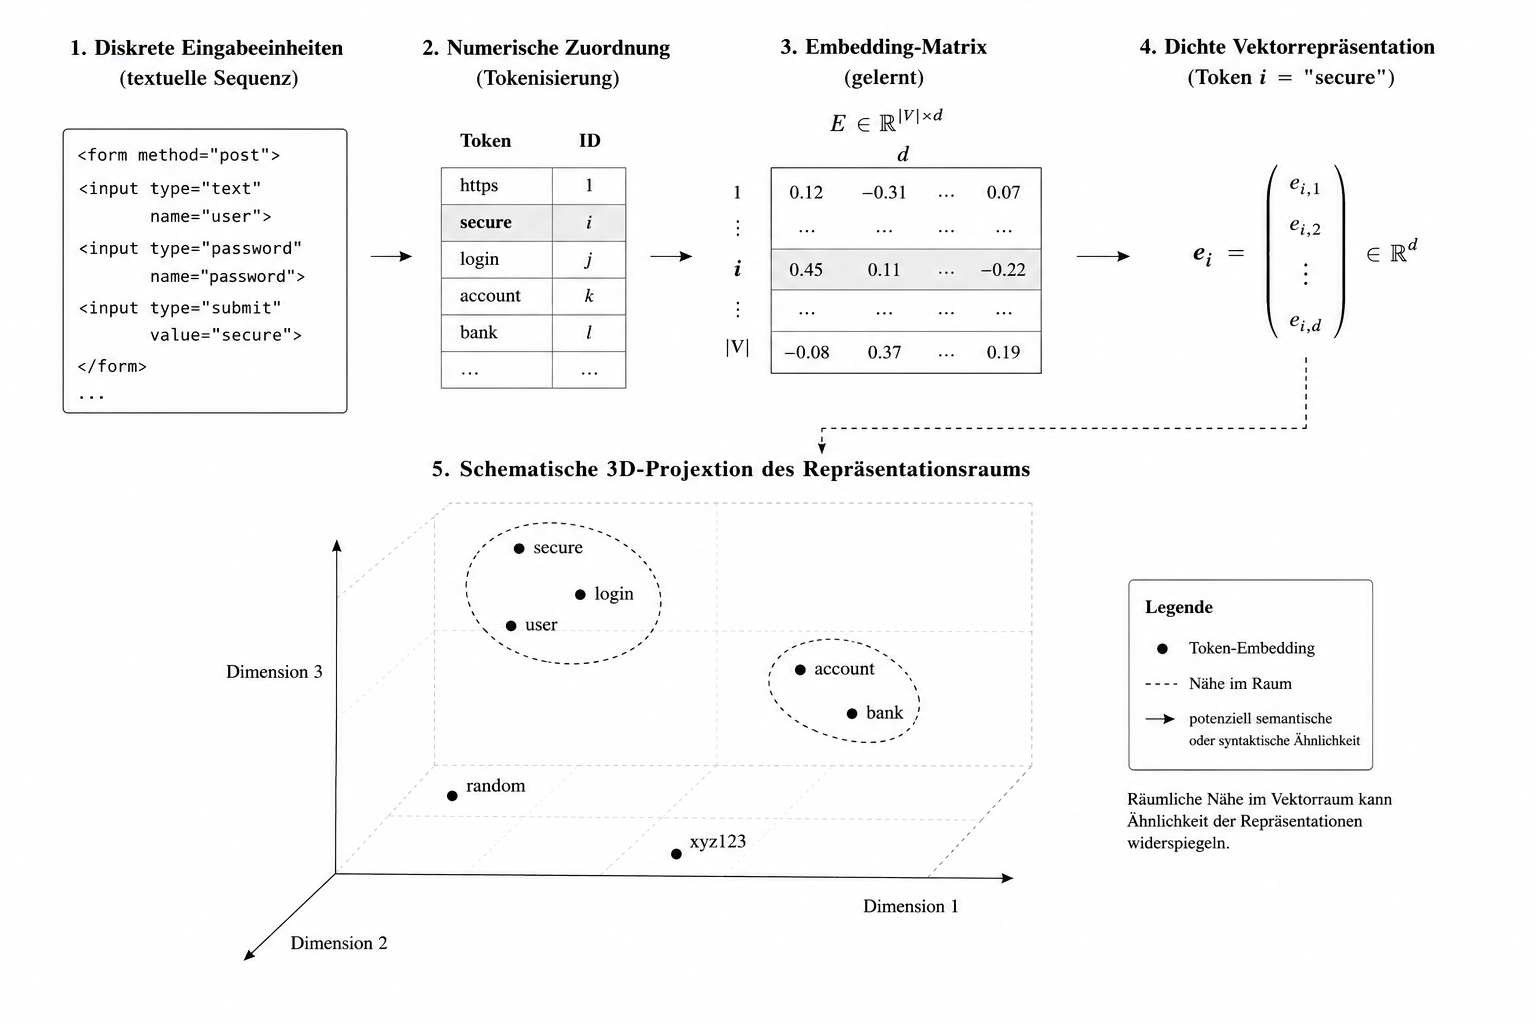
\includegraphics[width=\textwidth]
    {Praefix/Image/Vektorraum.png}

    \caption{Von diskreten Eingabeeinheiten zu gelernten Vektorrepräsentationen}
    \label{fig:vektorraum}
    \vspace{0.2em}

    {\footnotesize Quelle: (Eigene Darstellung nach [Collobert et al. (2011), S. 2501]; [Turney und Pantel (2010), S. 141 und 148]; [Mikolov et al. (2013), S. 1]); KI-unterstützt.}
\end{figure}

Die räumliche Anordnung in Abbildung~\ref{fig:vektorraum} verdeutlicht, dass
gelernte Vektorrepräsentationen über eine reine numerische Kennzeichnung
hinausgehen. Eine konzeptionelle Grundlage für die Interpretation
solcher Repräsentationsräume bildet die distributionelle Annahme, nach der
sprachliche Einheiten mit ähnlichen Verwendungskontexten tendenziell ähnliche
Bedeutungen aufweisen
(vgl. [Turney und Pantel (2010), S. 148]).
Auch gelernte Wortrepräsentationen können syntaktische und semantische Beziehungen
in ihren Vektoren abbilden
(vgl. [Mikolov et al. (2013), S. 1]).
Die dreidimensionale Darstellung in Abbildung \ref{fig:vektorraum} dient dabei
ausschließlich der schematischen Visualisierung eines tatsächlich
mehrdimensionalen Repräsentationsraums; die dargestellten Positionen und
Gruppierungen stellen keine empirisch ermittelten Repräsentationen des in dieser
Arbeit eingesetzten Modells dar.

Weitere parametrisierte Schichten können Eingaberepräsentationen schrittweise in höherstufige Merkmalsdarstellungen transformieren (vgl. [LeCun et al. (2015), S. 436]). Die Modellrepräsentation geht damit über die anfängliche Zuordnung eines Vektors zu einem Token hinaus.

Für die vorliegende Arbeit bildet dieses Prinzip die Grundlage für die Verarbeitung
der textuellen Eingabemodalitäten URL und HTML-Text. Die zusätzlich betrachtete
DOM-Struktur bildet demgegenüber explizite Beziehungen zwischen HTML-Elementen ab
und kann als Graph repräsentiert werden, in dem HTML-Elemente als Knoten und ihre
Eltern-Kind-Beziehungen als Kanten modelliert werden
(vgl. [Yoon et al. (2024), S. 9]). Neuronale und graphbasierte Verfahren zur
weiterführenden Repräsentationsbildung werden im folgenden Abschnitt betrachtet.

\subsection{Neuronale und graphbasierte Repräsentationsmodelle}

Neuronale Netze bestehen aus verbundenen Verarbeitungseinheiten mit trainierbaren Gewichten; verborgene Einheiten bilden interne Repräsentationen zwischen Ein- und Ausgabe (vgl. [Rumelhart et al. (1986), S.~533]).

Jede Einheit verarbeitet gewichtete Aktivierungen über eine Aktivierungsfunktion; die Gewichte werden anhand des Lernziels angepasst (vgl. [Rumelhart et al. (1986), S.~533]).

Deep Learning verbindet mehrere nichtlineare Verarbeitungsebenen, um geeignete Merkmale und aufeinander aufbauende Repräsentationen aus Daten zu erlernen (vgl. [Bengio (2009), S.~4--6]).


\begin{figure}[H]
    \centering

    \IfFileExists
    {Praefix/Image/NeuronaleNetze.png}
    {
        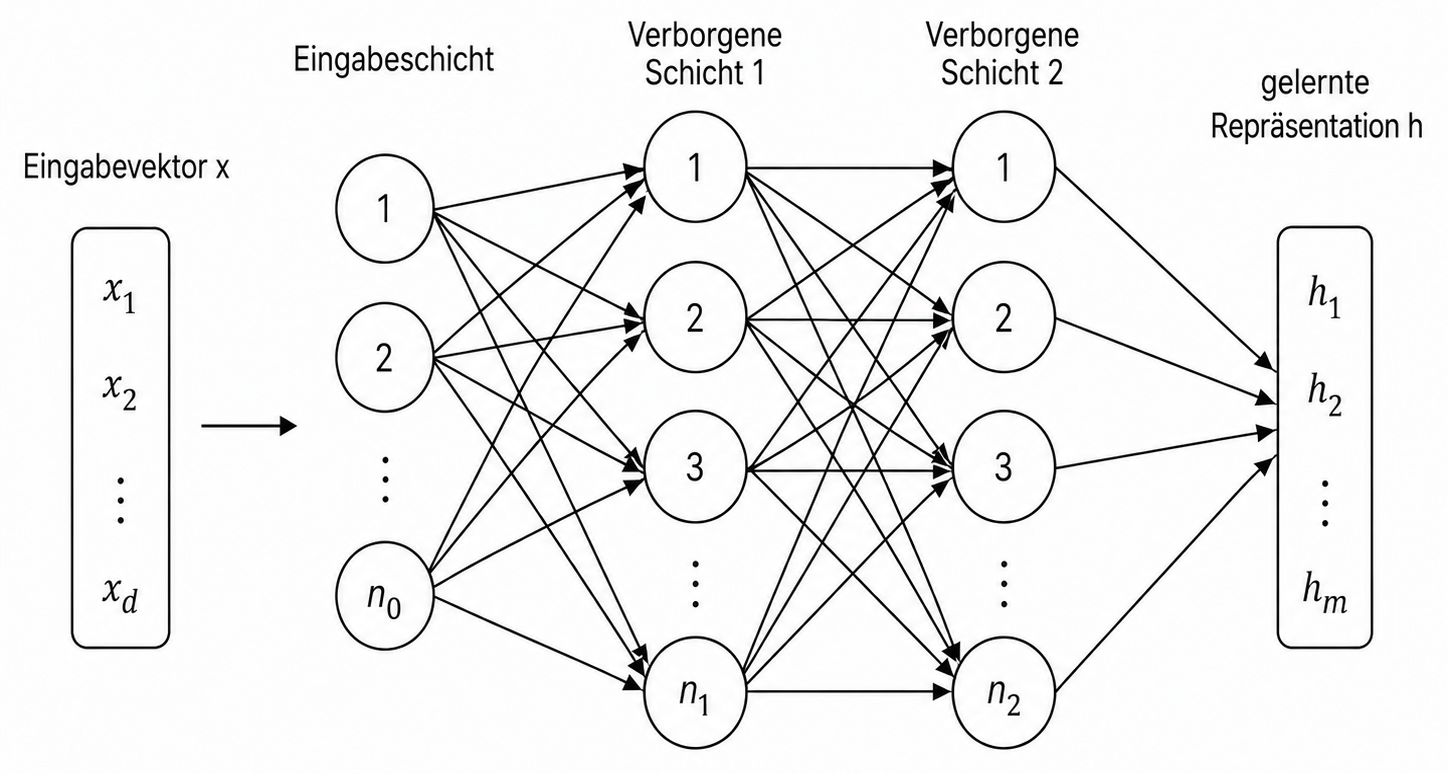
\includegraphics[width=\textwidth]
        {Praefix/Image/NeuronaleNetze.png}
    }
    {
        \fbox{
            \parbox[c][6.5cm][c]{0.92\textwidth}{
                \centering
                \textbf{Platzhalter Abbildung}\\[0.5em]
                Eingabevektor
                $\rightarrow$
                verborgene Schicht 1
                $\rightarrow$
                verborgene Schicht 2
                $\rightarrow$
                Ausgaberepräsentation
            }
        }
    }

    \caption{Schematischer Aufbau eines mehrschichtigen neuronalen Netzes}
    \label{fig:neuronale_repraesentationsbildung}
    \vspace{0.2em}

    {\footnotesize Quelle: (Eigene Darstellung nach [Rumelhart et al. (1986), S.~533]); KI-unterstützt.}
\end{figure}

Abbildung~\ref{fig:neuronale_repraesentationsbildung} zeigt eine vereinfachte mehrschichtige Verarbeitung. Zusätzliche verborgene Ebenen ermöglichen zunehmend abstrakte Merkmalsdarstellungen (vgl. [Bengio (2009), S. 4--6]).

Graphen ergänzen Knotenmerkmale um explizite Beziehungen zwischen den Knoten, die als Kanten dargestellt werden (vgl. [Kipf und Welling (2017), S. 1]).

Graph Convolutional Networks (GCNs) bilden Knotenrepräsentationen unter Berücksichtigung der eigenen Merkmale und der lokalen Nachbarschaft (vgl. [Kipf und Welling (2017), S. 1--2]). Mehrere Verarbeitungsschichten beziehen entsprechend weiter entfernte Nachbarschaften ein (vgl. [Kipf und Welling (2017), S. 3]).

Für Webseiten lässt sich dieses Prinzip auf die DOM-Struktur eines
HTML-Dokuments übertragen. HTML-Elemente können dabei als Knoten und ihre
hierarchischen Eltern-Kind-Beziehungen als Kanten eines Graphen modelliert
werden
(vgl. [Yoon et al. (2024), S. 9]).
Dadurch können neben den Eigenschaften einzelner HTML-Elemente auch deren
strukturelle Beziehungen in die Repräsentationsbildung einbezogen werden.

\begin{figure}[H]
    \centering
    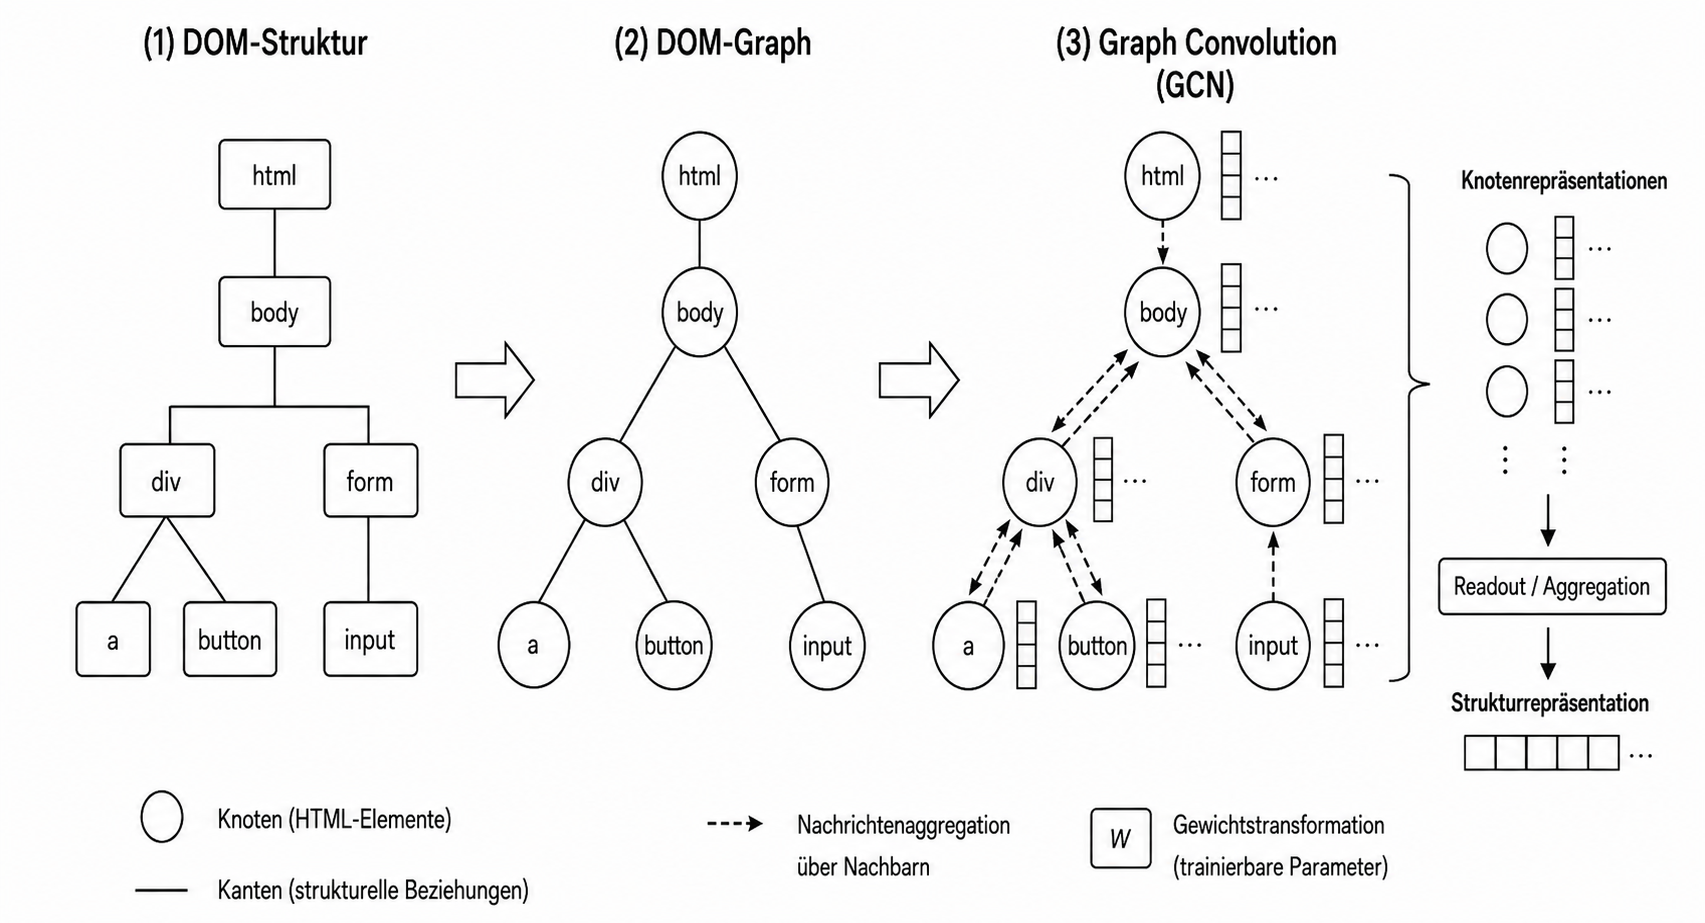
\includegraphics[
        width=1.0\textwidth,
        height=1.0\textheight,
        keepaspectratio
    ]{Praefix/Image/DOMDarstellung.png}
    \caption{Schematische graphbasierte Repräsentationsbildung einer DOM-Struktur}
    \label{fig:dom_gcn_repraesentationsbildung}
    \vspace{0.2em}

    {\footnotesize Quelle: (Eigene Darstellung nach [Kipf und Welling (2017), S. 1--3]; [Yoon et al. (2024), S. 9 und 13]); KI-unterstützt.}
\end{figure}

Abbildung \ref{fig:dom_gcn_repraesentationsbildung} veranschaulicht die
graphbasierte Verarbeitung dieser DOM-Struktur. Ein GCN kann dabei
Knotenmerkmale gemeinsam mit der lokalen Graphstruktur verarbeiten und daraus
strukturabhängige Repräsentationen erzeugen
(vgl. [Kipf und Welling (2017), S. 1--2]).

Damit stehen für die weitere Modellierung unterschiedliche Formen der
Repräsentationsbildung zur Verfügung. URL und HTML-Text werden als
sequenzielle Eingaben verarbeitet, während der DOM die explizite Struktur
des HTML-Dokuments graphbasiert abbildet. Für die kontextabhängige
Verarbeitung der sequenziellen Eingaben werden in der vorliegenden Arbeit
transformerbasierte Encodermodelle eingesetzt, die im folgenden Abschnitt
betrachtet werden.

\subsection{Transformerbasierte Repräsentationsmodelle}
\label{sec:transformerbasierte_repraesentationsmodelle}

Die ursprüngliche Transformer-Architektur besteht aus Encoder und Decoder; der Encoder überführt Eingabesequenzen in kontextabhängige Repräsentationen, die der Decoder für seine Ausgaben nutzt (vgl. [Vaswani et al. (2017), S. 2]). Da die Architektur ohne Rekurrenz und Faltung auskommt, werden den Embeddings Positionsinformationen hinzugefügt (vgl. [Vaswani et al. (2017), S. 6]).

Attention bildet Query-, Key- und Value-Vektoren und gewichtet Values anhand der Ähnlichkeit von Queries und Keys (vgl. [Vaswani et al. (2017), S. 3--4]). Für Scaled Dot-Product Attention gilt (vgl. [Vaswani et al. (2017), S. 4]):

\begin{equation*}
\mathrm{Attention}(Q,K,V)
=
\mathrm{softmax}
\left(
\frac{QK^{T}}{\sqrt{d_k}}
\right)V
\end{equation*}

\begin{center}
    \footnotesize{Quelle: (vgl. [Vaswani et al. (2017), S. 4]).}
\end{center}

\begin{description}
    \item[\textbf{$Q$ (Query):}]
    Repräsentiert die Anfragen, anhand derer bestimmt wird, welche
    Informationen anderer Sequenzpositionen für die jeweils betrachtete
    Position relevant sind.

    \item[\textbf{$K$ (Key):}]
    Enthält die Schlüsselrepräsentationen der Sequenzpositionen, mit denen
    die Queries zur Bestimmung ihrer jeweiligen Relevanz verglichen werden.

    \item[\textbf{$V$ (Value):}]
    Enthält die zu den Sequenzpositionen gehörenden Informationen, die
    entsprechend der berechneten Attention-Gewichte in die neue
    Repräsentation einfließen.

    \item[\textbf{$d_k$:}]
    Bezeichnet die Dimension der Key-Vektoren und dient als
    Skalierungsfaktor für die berechneten Skalarprodukte.
\end{description}

Die Skalarprodukte werden durch $\sqrt{d_k}$ skaliert, mittels Softmax normalisiert und zur gewichteten Kombination der Values verwendet (vgl. [Vaswani et al. (2017), S. 4]). Bei Self-Attention stammen Queries, Keys und Values aus derselben Sequenz (vgl. [Vaswani et al. (2017), S. 5]). Multi-Head Attention berechnet mehrere solcher Ausgaben mit eigenen Projektionen und führt sie anschließend zusammen (vgl. [Vaswani et al. (2017), S. 4--5]).

Im Encoder folgen auf Multi-Head Attention positionsweise Feed-Forward-Netze; beide Teilkomponenten besitzen Residualverbindungen und Layer-Normalisierung (vgl. [Vaswani et al. (2017), S. 3 und 5]).

Bidirectional Encoder Representations from Transformers (BERT) verwendet einen mehrschichtigen Transformer-Encoder, dessen Attention den Kontext auf beiden Seiten einer Tokenposition berücksichtigt (vgl. [Devlin et al. (2019), S. 4171 und 4173]). Für Klassifikation kann der abschließende Hidden State des speziellen Tokens \texttt{[CLS]} als Sequenzrepräsentation dienen (vgl. [Devlin et al. (2019), S. 4174]).

Neben der Feinabstimmung des Encoders beschreiben Devlin et al. einen feature-basierten Ansatz, bei dem extrahierte Aktivierungen als feste Merkmale nachgelagerter Modelle dienen (vgl. [Devlin et al. (2019), S. 4179]). Die vorliegende Arbeit nutzt diese Trennung für die Repräsentationsvergleiche.

RoBERTa verändert das BERT-Vortraining unter anderem durch umfangreicheres Training, größere Datenmengen, dynamische Maskierung und den Verzicht auf Next Sentence Prediction (vgl. [Liu et al. (2019), S. 1]). Abschnitt~2.3 erläutert die hier relevanten selbstüberwachten Lernziele.

In der vorliegenden Arbeit werden transformerbasierte Encoder für die
beiden sequenziellen Informationsquellen URL und HTML-Text eingesetzt.
Der URL-Zweig basiert auf BERT, während für den HTML-Text ein
RoBERTa-Encoder verwendet wird. Die daraus erzeugten
kontextabhängigen Repräsentationen bilden die Grundlage für die
nachfolgenden selbstüberwachten Repräsentationsvarianten und deren
kontrollierte Downstream-Evaluation.

\subsection{Downstream-Klassifikation und multimodale Verarbeitung}

Die Downstream-Aufgabe dieser Arbeit ist die überwachte Klassifikation einer Webseite als Phishing oder legitim. Eine Linear Probe trainiert einen linearen Klassifikator auf eingefrorenen Repräsentationen, um deren Nutzbarkeit zu bewerten (vgl. [Chen et al. (2020), PDF-S.~3]). Mehrschichtige Netze sind dagegen nicht auf lineare Entscheidungsregionen beschränkt; Cybenkos Approximationsresultat gilt dabei für ausreichend große Netze mit geeigneten sigmoiden Aktivierungen (vgl. [Cybenko (1989), S.~303]). Der empirische Vergleich mit einer nichtlinearen Probe prüft, wie stark die gemessenen Repräsentationsunterschiede vom Klassifikationsmechanismus abhängen.

Multimodale Fusion integriert Informationen mehrerer Modalitäten für eine gemeinsame Vorhersage; merkmalsbasierte Fusion verbindet Repräsentationen vor der Entscheidung, entscheidungsbasierte Fusion dagegen die Ausgaben getrennter Modelle (vgl. [Baltrušaitis et al. (2019), S.~12]). Für URL, HTML-Text und DOM wird hier eine merkmalsbasierte Fusion eingesetzt.

Lernbare Modalitätsgewichte können über Softmax normalisiert und zur gewichteten Summe der Repräsentationen verwendet werden (vgl. [Zhou et al. (2019), PDF-S. 1--2]). Andere Architekturen nutzen abweichende Gating-Funktionen, beispielsweise sigmoide Gated Multimodal Units (vgl. [Arevalo et al. (2017), S.~5]). Eine zusätzliche Entwurfsdimension ist die Kaskadierung: Frühe Stufen schließen einen Teil der Eingaben ab, während verbleibende Fälle aufwendigere Stufen durchlaufen (vgl. [Viola und Jones (2004), S.~144]).



\section{Self-Supervised Representation Learning}
Self-Supervised Representation Learning leitet Trainingsziele aus den Eingabedaten selbst ab; eine solche Hilfsaufgabe (\textit{Pretext Task}) benötigt keine manuell annotierten Zielwerte der späteren Aufgabe (vgl. [Ericsson et al. (2022), S. 42--43]). Die vortrainierten Repräsentationen können anschließend als feste Merkmale oder durch weitere Feinabstimmung für eine \textit{Downstream Task} genutzt werden (vgl. [Ericsson et al. (2022), S. 44--45]).

Abbildung \ref{fig:ssrl_grundprinzip} veranschaulicht diese Trennung
zwischen selbstüberwachtem Vortraining und nachgelagerter Nutzung der
erlernten Repräsentationen.

\begin{figure}[H]
    \centering

    \begin{tikzpicture}[
        font=\footnotesize,
        >={Latex[length=2.1mm]},
        topbox/.style={
            draw=black,
            line width=0.55pt,
            align=center,
            text width=3.1cm,
            minimum height=2.9cm,
            inner sep=4pt
        },
        box/.style={
            draw=black,
            line width=0.55pt,
            align=center,
            text width=3.1cm,
            minimum height=1.9cm,
            inner sep=4pt
        },
        arrow/.style={
            ->,
            line width=0.65pt
        },
        node distance=0.6cm
    ]

    % Obere Reihe
    \node[topbox] (data) {
        \textbf{Ungelabelte Daten}\\[3pt]
        z.\,B. Texte, Webseiten\\
        oder Dokumente
    };

    \node[topbox, right=of data] (pretext) {
        \textbf{Selbstüberwachtes}\\
        \textbf{Lernziel}\\
        \textit{(Pretext Task)}\\[3pt]
        z.\,B. Maskierung oder\\
        kontrastive Paarung
    };

    \node[topbox, right=of pretext] (encoder) {
        \textbf{Encoder / Vortraining}\\[3pt]
        Lernen einer\\
        übertragbaren\\
        Repräsentations-\\
        funktion
    };

    % Untere Reihe
    \node[
        box,
        below=0.75cm of encoder
    ] (representation) {
        \textbf{Gelernte}\\
        \textbf{Repräsentation}\\[3pt]
        Übertragbare\\
        Merkmalsdarstellung
    };

    \node[
        box,
        right=of representation
    ] (downstream) {
        \textbf{Downstream-Aufgabe}\\
        \textit{(mit Labels)}\\[3pt]
        z.\,B. Klassifikation
    };

    % Pfeile
    \draw[arrow] (data.east) -- (pretext.west);
    \draw[arrow] (pretext.east) -- (encoder.west);
    \draw[arrow] (encoder.south) -- (representation.north);
    \draw[arrow] (representation.east) -- (downstream.west);

    \end{tikzpicture}

    \caption{Grundprinzip des Self-Supervised Representation Learning}
    \label{fig:ssrl_grundprinzip}
    \vspace{0.2em}

    {\footnotesize Quelle: (Eigene Darstellung nach [Ericsson et al. (2022), S. 42--46]); KI-unterstützt.}
\end{figure}

Die Wahl der Pretext-Aufgabe bestimmt das Trainingssignal und beeinflusst die erlernte Repräsentation (vgl. [Ericsson et al. (2022), S. 42--43]). Im Folgenden werden maskierte und kontrastive Lernziele sowie die task-adaptive Weiteranpassung unterschieden.

\subsection{Maskierte selbstüberwachte Lernziele}

Masked Language Modeling (MLM) trainiert einen Encoder darauf, ausgewählte Token aus dem verbleibenden beidseitigen Kontext zu rekonstruieren; die ursprünglichen Token liefern dabei die Zielwerte ohne manuelle Klassenannotation (vgl. [Devlin et al. (2019), S.~4172 und 4174]).

BERT wählt 15~\% der Tokenpositionen aus, ersetzt davon 80~\% durch das Maskierungstoken und 10~\% durch zufällige Token und belässt 10~\% unverändert; für diese Positionen wird jeweils das ursprüngliche Token vorhergesagt (vgl. [Devlin et al. (2019), S.~4174]). Auch RoBERTa nutzt MLM als Vortrainingsziel (vgl. [Gururangan et al. (2020), S.~8343]).

Das grundlegende Zusammenspiel aus Maskierung, kontextabhängiger
Repräsentationsbildung und Rekonstruktion ist in Abbildung~\ref{fig:mlm-konzept}
exemplarisch für eine HTML-Textsequenz dargestellt.

\begin{figure}[H]
    \centering
    % KI-unterstuetzte eigene schematische Darstellung; keine gemessenen Tokenfolgen.
\begin{tikzpicture}[font=\small,>=stealth,
  box/.style={draw,rounded corners=2pt,align=center,minimum height=.8cm,text width=11cm}]
\node[box] (input) {Bereinigter HTML-Text: \texttt{Secure Login -- Verify your account}};
\node[box,above=0.5cm of input] (masked) {Maskierte Eingabe: \texttt{<mask> Login -- Verify your <mask>}};
\node[box,above=0.5cm of masked] (encoder) {RoBERTa-Encoder: kontextabhängige Tokenrepräsentationen};
\node[box,above=0.5cm of encoder] (head) {MLM-Head: Vorhersage der ursprünglichen ausgewählten Token};
\node[above=0.35cm of head,align=center] (target) {Schematische Vorhersageziele: \texttt{Secure}, \texttt{account}};
\draw[->] (input)--(masked);
\draw[->] (masked)--(encoder);
\draw[->] (encoder)--(head);
\draw[->] (head)--(target);
\end{tikzpicture}

    \caption{Schematisches Prinzip des Masked Language Modeling am Beispiel des HTML-Textzweigs}
    \label{fig:mlm-konzept}
    \vspace{0.2em}

    {\footnotesize Quelle: (Eigene Darstellung nach [Devlin et al. (2019), S.~4174]; [Gururangan et al. (2020), S.~8343]); KI-unterstützt.}
\end{figure}

Abbildung~\ref{fig:mlm-konzept} überträgt MLM auf den HTML-Textzweig. Die Wörter sind schematisch; im Code werden Subword-Token maskiert und rekonstruiert. MLM kann auch das Vortraining auf weiteren ungelabelten Daten fortsetzen (vgl. [Gururangan et al. (2020), S.~8343]). Abschnitt~2.3.3 behandelt die aufgabenbezogene Fortsetzung.

\subsection{Kontrastives Repräsentationslernen}

Kontrastives Lernen nähert Repräsentationen positiver Paare einander an und unterscheidet sie von negativen Vergleichsinstanzen; für Text kann dies mit vortrainierten Transformer-Encodern umgesetzt werden (vgl. [Gao et al. (2021), S.~6895]).

Die Ähnlichkeit zweier Repräsentationen kann dabei über die
Kosinusähnlichkeit bestimmt werden. Innerhalb der kontrastiven
Verlustfunktion beeinflusst ein Temperaturparameter die Skalierung der
Ähnlichkeitswerte. Das Lernziel begünstigt dadurch eine hohe Ähnlichkeit
positiver Paare relativ zu den verfügbaren negativen Vergleichsinstanzen
(vgl. [Gao et al. (2021), S.~6895]).
\begin{figure}[H]
    \centering
    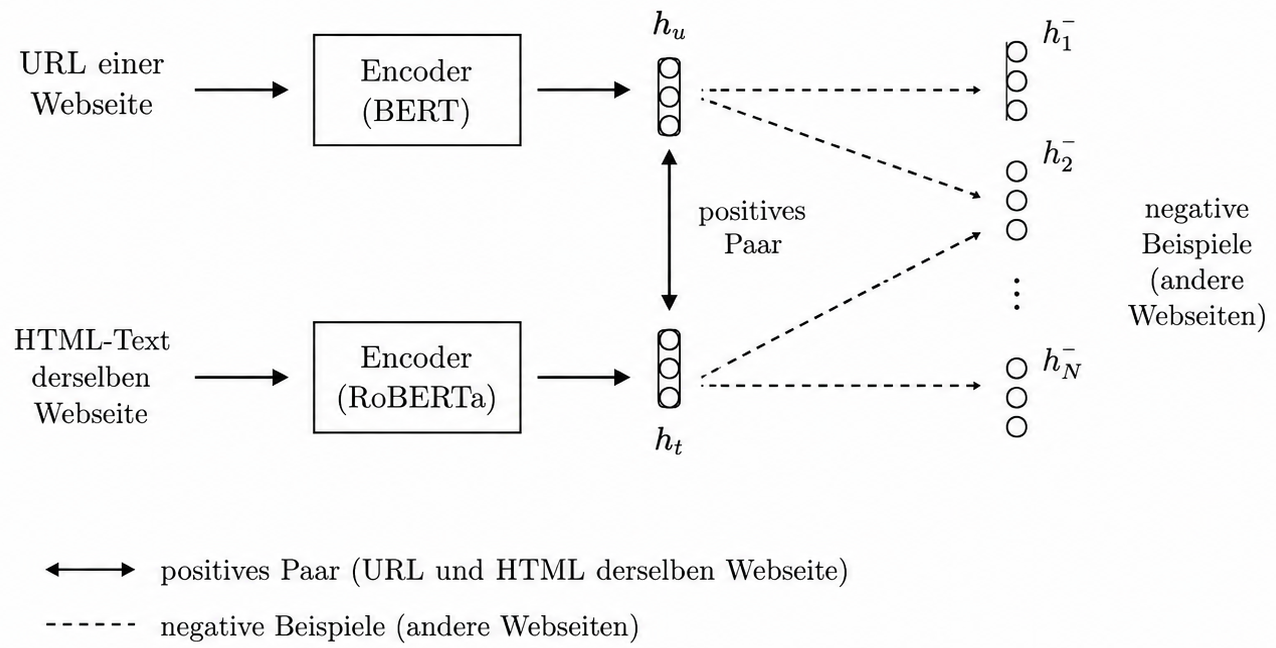
\includegraphics[width=0.72\textwidth]{Praefix/Image/ContrastiveKonzept.png}
    \caption{Schematisches Prinzip des kontrastiven Repräsentationslernens für URL--HTML-Paare}
    \label{fig:contrastive-konzept}
    \vspace{0.2em}

    {\footnotesize Quelle: (Eigene Darstellung nach [Gao et al. (2021), S.~6895]); Übertragung auf URL--HTML-Paare, KI-unterstützt.}
\end{figure}

Ergänzend wird kontrastives Repräsentationslernen als alternative
selbstüberwachte Zielfunktion betrachtet. URL und HTML-Text derselben Webseite
bilden dabei ein positives Paar, während Repräsentationen anderer Webseiten als
negative Beispiele dienen. Das Trainingssignal entsteht somit ohne Verwendung
von Phishing- oder Benign-Labels. Die konkrete Umsetzung wird in
Abschnitt~4.3.2 beschrieben.

\subsection{Task-Adaptive Pretraining}

Task-Adaptive Pretraining (TAPT) setzt das RoBERTa-Vortraining auf dem ungelabelten Trainingskorpus einer konkreten Downstream-Aufgabe fort (vgl. [Gururangan et al. (2020), S. 8346]).

Die angepassten Repräsentationen werden anschließend für das überwachte Training der Zielaufgabe verwendet (vgl. [Gururangan et al. (2020), S. 8346]).

Die Trennung beider Lernphasen lässt sich vereinfacht wie folgt darstellen:

\begin{equation}
\theta_{\mathrm{pre}}
\xrightarrow[\mathcal{D}^{\mathrm{unlabeled}}_{\mathrm{task}}]
{\mathcal{L}_{\mathrm{MLM}}}
\underbrace{\theta_{\mathrm{TAPT}}}_{\text{Task-Adaptive Pretraining}}
\rightarrow
\theta_{\mathrm{TAPT}}
\xrightarrow[\mathcal{D}^{\mathrm{labeled}}_{\mathrm{task}}]
{\mathcal{L}_{\mathrm{cls}}}
\underbrace{\theta_{\mathrm{task}}}_{\text{Downstream-Training}} .
\end{equation}

\begin{center}
    \footnotesize{Quelle: (Eigene Darstellung nach [Gururangan et al. (2020), S.~8346]); KI-unterstützt.}
\end{center}

Domain-Adaptive Pretraining (DAPT) nutzt dagegen einen breiteren ungelabelten Korpus der Domäne; TAPT ist durch die Auswahl der Trainingsdaten enger an eine konkrete Zielaufgabe gebunden (vgl. [Gururangan et al. (2020), S. 8342--8343 und 8346]).

In der vorliegenden Arbeit wird TAPT auf die beiden sequenziellen Informationsquellen URL und
HTML-Text übertragen. Die vortrainierten Encoder werden hierzu getrennt mittels MLM auf dem
ungelabelten Webseiten-Trainingspool weiter angepasst. Da derselbe Pool anschließend die
Ausgangsbasis der gelabelten Downstream-Budgets bildet, entspricht dieser Versuchsaufbau der
task-adaptiven Variante. Dadurch lassen sich die isolierte Anpassung einzelner
Informationsquellen sowie ihre gemeinsame Anpassung gegenüber nicht adaptierten
Repräsentationen unter unterschiedlichen Labelbudgets und Evaluationsbedingungen untersuchen.
\section{Evaluationsrahmen und Bewertungsmetriken}
\label{sec:evaluation_metrics}

\subsection{Klassifikations- und Betriebspunktmetriken}

\paragraph{True-Positive-Rate, False-Positive-Rate und Precision}
Bei einer binären Klassifikation ergeben sich aus tatsächlicher und vorhergesagter Klasse
die vier Fälle True Positive (TP), False Positive (FP), True Negative (TN) und False
Negative (FN). Darauf aufbauend lassen sich True-Positive-Rate (TPR),
False-Positive-Rate (FPR) und Precision bestimmen
(vgl. [Saito und Rehmsmeier (2015), S. 3--4]):

\[
\mathrm{TPR}=\frac{TP}{TP+FN},
\qquad
\mathrm{FPR}=\frac{FP}{FP+TN},
\qquad
\mathrm{Precision}=\frac{TP}{TP+FP}.
\]

\begin{center}
\footnotesize Quelle: (vgl. [Saito und Rehmsmeier (2015), S. 4]).
\end{center}

TPR entspricht dem Recall, FPR dem Anteil falsch positiver unter allen negativen Instanzen und Precision dem Anteil tatsächlich positiver unter allen positiven Vorhersagen (vgl. [Saito und Rehmsmeier (2015), S. 4]). In dieser Arbeit ist Phishing die positive und legitim die negative Klasse.

\paragraph{Betriebspunkt} Die Klassifikationsschwelle bestimmt das Verhältnis von TPR und FPR (vgl. [Saito und Rehmsmeier (2015), S. 4]). Für die Phishing-Erkennung sind insbesondere Betriebspunkte mit niedriger FPR relevant (vgl. [Purwanto et al. (2022), S. 1506]).

Die vorliegende Arbeit betrachtet deshalb primär die TPR an einem festgelegten
Low-FPR-Betriebspunkt und die dort realisierte FPR. Ergänzend wird mit
$\mathrm{FPR@TPR90}$ die umgekehrte Perspektive verwendet: Sie gibt an, welche
False-Positive-Rate am ersten empirischen ROC-Punkt mit einer TPR von mindestens
90\,\% erreicht wird. Eine Interpolation auf exakt 90\,\% erfolgt nicht.
Niedrigere Werte entsprechen dabei einer günstigeren Trennung der beiden Klassen.
Beide Perspektiven erlauben damit eine Bewertung der Klassifikationsleistung bei
kontrollierter Erkennungs- beziehungsweise Fehlalarmrate.

\paragraph{Ergänzende Precision-Recall-Metriken}
Neben einzelnen Betriebspunkten kann die Modellleistung über unterschiedliche
Klassifikationsschwellen betrachtet werden. Die Precision-Recall-Kurve stellt hierzu
Precision und Recall über verschiedene Schwellenwerte gegenüber
(vgl. [Saito und Rehmsmeier (2015), S. 4 und 7]). Die Average Precision (AP) fasst
diese Rankingperspektive über die Kurve zusammen. Dalton et al. verwenden im
PhreshPhish-Benchmark ergänzend eine als Precision bei 90\,\% Recall bezeichnete
Kennzahl ($P@R=0{,}90$) (vgl. [Dalton et al. (2026), S. 7]).

Precision und darauf aufbauende Precision-Recall-Metriken hängen zusätzlich von der
Klassenverteilung der Evaluationsmenge ab
(vgl. [Saito und Rehmsmeier (2015), S. 5 und 7]). AP und der nachfolgend präzisierte
Kennwert $P_{\geq 90}$ werden in der
vorliegenden Arbeit daher ergänzend zur Beschreibung der Rankingqualität auf einem
festen Evaluationsbestand verwendet. Die zentralen Modell- und Systemvergleiche
stützen sich dagegen auf TPR und FPR an den festgelegten Betriebspunkten.
Der implementierte Kennwert $P_{\geq 90}$ ist die maximale Precision unter allen
empirischen Schwellen mit Recall von mindestens 90\,\%:
\[
P_{\geq 90}=\max_{\tau:\,\mathrm{TPR}(\tau)\geq 0{,}90}
\mathrm{Precision}(\tau).
\]
Er bezeichnet somit keine interpolierte Precision bei exakt 90\,\% Recall.
AP wird als Summe der Precision-Werte gewichtet mit den jeweiligen Recall-Zuwächsen
berechnet; sie entspricht hier keiner trapezförmigen Flächenintegration.


\subsection{Generalisierung unter Distribution Shift}

Eine besondere Herausforderung für die Generalisierung lernbasierter Modelle
entsteht, wenn sich die zugrunde liegende Datenverteilung zwischen Training und
späterer Evaluation verändert. Koh et al. bezeichnen als Distribution Shift
Situationen, in denen sich Trainings- und Testverteilung unterscheiden
(vgl. [Koh et al. (2021), PDF-S. 1]). Vereinfacht lässt sich dieser Zusammenhang
durch

\[
P_{\mathrm{train}}(X,Y) \neq P_{\mathrm{test}}(X,Y)
\]

beschreiben, wobei \(X\) die Eingabedaten und \(Y\) die zugehörige Zielklasse
bezeichnet. Koh et al. zeigen anhand mehrerer realer Datensätze, dass Modelle
unter solchen Out-of-Distribution-Bedingungen deutlich geringere Leistungen
als unter vergleichbaren Trainings- und Testbedingungen erreichen können
(vgl. [Koh et al. (2021), PDF-S. 1--2]).

Zeitliche Veränderungen und zuvor unbeobachtete Domänen bilden mögliche Ursachen von Verteilungsverschiebungen; WILDS berücksichtigt beide Formen in seinen Testbedingungen (vgl. [Koh et al. (2021), PDF-S.~1--3]).

Für die vorliegende Arbeit bildet diese Unterscheidung die theoretische
Grundlage für die spätere Evaluation unter veränderten Datenbedingungen.
Die konkrete Konstruktion der verwendeten Testszenarien und die Festlegung des
Low-FPR-Betriebspunkts werden in Abschnitt~4.4.1 beschrieben.

\subsection{Statistische Auswertungsverfahren}

Stochastisches Training kann zwischen Läufen unterschiedliche Ergebnisse erzeugen; Reimers und Gurevych empfehlen deshalb die Bewertung mehrerer Ausführungen anstelle einzelner Ergebniswerte (vgl. [Reimers und Gurevych (2017), S.~338]).

\paragraph{Gepaarte Leistungsdifferenzen}
Werden zwei Modellvarianten unter korrespondierenden Bedingungen verglichen,
können die jeweils zusammengehörigen Beobachtungen paarweise gegenübergestellt
werden. Holt und Sullivan bilden hierfür die Differenzen zwischen den
Beobachtungspaaren und verwenden deren Mittelwert als Teststatistik
(vgl. [Holt und Sullivan (2023), S.~787--788]):

\begin{equation*}
d_i=x_i-y_i,
\qquad
T=\bar{d}.
\end{equation*}

\begin{center}
    \footnotesize{Quelle: (vgl. [Holt und Sullivan (2023), S.~787--788]).}
\end{center}

Die Paarbildung erhält die Zuordnung korrespondierender Beobachtungen (vgl. [Holt und Sullivan (2023), S.~787--788]). Differenzen prozentual ausgewiesener Metriken werden in dieser Arbeit in Prozentpunkten berichtet.

\paragraph{Konfidenzintervalle} Konfidenzintervalle ergänzen Punktschätzungen um eine Unsicherheitsangabe, häufig zum Niveau von 95~\% oder 99~\% (vgl. [Botsch (2023), S. 15]). Hier beschreiben 95-\%-Intervalle die Unsicherheit mittlerer Differenzen aus gepaarten Downstream-Wiederholungen; ihre Interpretation setzt die in Kapitel~4 genannten Bedingungen voraus.

Bootstrap-Resampling zieht wiederholt Stichproben gleicher Größe mit Zurücklegen und berechnet die Leistungsmetrik erneut (vgl. [Raschka (2018), S. 16]). Beim 95-\%-Percentile-Intervall bilden das 2,5-\%- und 97,5-\%-Quantil der Bootstrap-Verteilung die Grenzen (vgl. [Raschka (2018), S. 18]).

\paragraph{Exakter Sign-Flip-Permutationstest} Bei unter der Nullhypothese um null symmetrischen Paardifferenzen lässt sich eine Nullverteilung ihres Mittelwerts durch alle Vorzeichenkombinationen bilden (vgl. [Holt und Sullivan (2023), S. 787--788]).

Für $n$ Paare gibt es $2^n$ Vorzeichenkombinationen; der zweiseitige exakte $p$-Wert ist deren Anteil mit einem mindestens so großen absoluten Mittelwert wie beobachtet (vgl. [Holt und Sullivan (2023), S. 788]).

\paragraph{Korrektur multipler Tests} Mit mehreren Hypothesentests kann das Risiko mindestens einer falschen Zurückweisung innerhalb der Testfamilie steigen (vgl. [Dror et al. (2017), S.~471 und 474]).

Die Holm-Prozedur sortiert $m$ $p$-Werte aufsteigend und vergleicht sie nacheinander mit $\alpha/(m-i+1)$, bis erstmals keine Zurückweisung erfolgt; dadurch wird die familienbezogene Fehlerwahrscheinlichkeit kontrolliert (vgl. [Holm (1979), S.~66--67]).

In der vorliegenden Arbeit werden die Größenordnung der beobachteten
Leistungsunterschiede, die Unsicherheit ihrer Schätzung und die Ergebnisse der
statistischen Tests gemeinsam berichtet. Die konkrete Anzahl der Wiederholungen,
die Paarbildung sowie die Zuordnung mehrerer Vergleiche zu gemeinsamen
Testfamilien werden im Methodikkapitel festgelegt.

\subsection{Effizienz- und Betriebsmetriken}

Die technische Evaluation berücksichtigt neben der Klassifikationsgüte auch den Inferenzaufwand. Reddi et al. unterscheiden latenzorientierte Szenarien und durchsatzorientierte Batch-Verarbeitung (vgl. [Reddi et al. (2020), S.~5--6]).

\begin{itemize}
    \item \textbf{Median-Latenz [ms]:}
    bezeichnet in dieser Arbeit das 50.\ Perzentil der gemessenen
    Inferenzzeiten und beschreibt damit die typische Verarbeitungsdauer
    einer Eingabe.

    \item \textbf{95.\ Perzentil der Latenz [ms]:}
    bezeichnet den Latenzwert, den 95\,\% der beobachteten
    Inferenzvorgänge nicht überschreiten. Perzentilbasierte
    Latenzmetriken werden auch in etablierten Inferenzbenchmarks zur
    Betrachtung langsamerer Bereiche der Laufzeitverteilung eingesetzt
    (vgl. [Reddi et al. (2020), S.~5--6]).

    \item \textbf{Durchsatz [Seiten/s]:}
    beschreibt die Anzahl der innerhalb eines Zeitraums verarbeiteten
    Eingaben. Im Offline-Szenario des MLPerf-Inference-Benchmarks wird
    entsprechend der Durchsatz in Samples pro Sekunde betrachtet
    (vgl. [Reddi et al. (2020), S.~6]).

    \item \textbf{Peak-VRAM [MiB]:}
    bezeichnet in dieser Arbeit den maximal während des betrachteten
    Inferenzpfads belegten GPU-Speicher.

    \item \textbf{Eskalationsrate [\%]:}
    bezeichnet bei einer kaskadierten Verarbeitung den Anteil der Eingaben,
    für die nach der ersten Verarbeitungsstufe zusätzlich der vollständige
    multimodale Modellpfad ausgeführt wird.
\end{itemize}

Latenz und Durchsatz erfassen unterschiedliche Aspekte der technischen
Verarbeitung und sind daher gemeinsam zu betrachten
(vgl. [Reddi et al. (2020), S.~11]). Peak-VRAM und Eskalationsrate ergänzen
diese Kennzahlen um den Ressourcenbedarf und den Verarbeitungsumfang.

